\chapter{Introduction}\label{chapter:introduction}

\section{First Section of My Introduction}

\subsection{Key Motivations for this Research}
Finding any motivation to conduct research is left as an exercise for the reader.

Say some things and cite some things.

\texttt{Astropy} is helpful astronomy software \citep{astropy2022}.

\begin{figure}
    \centering
	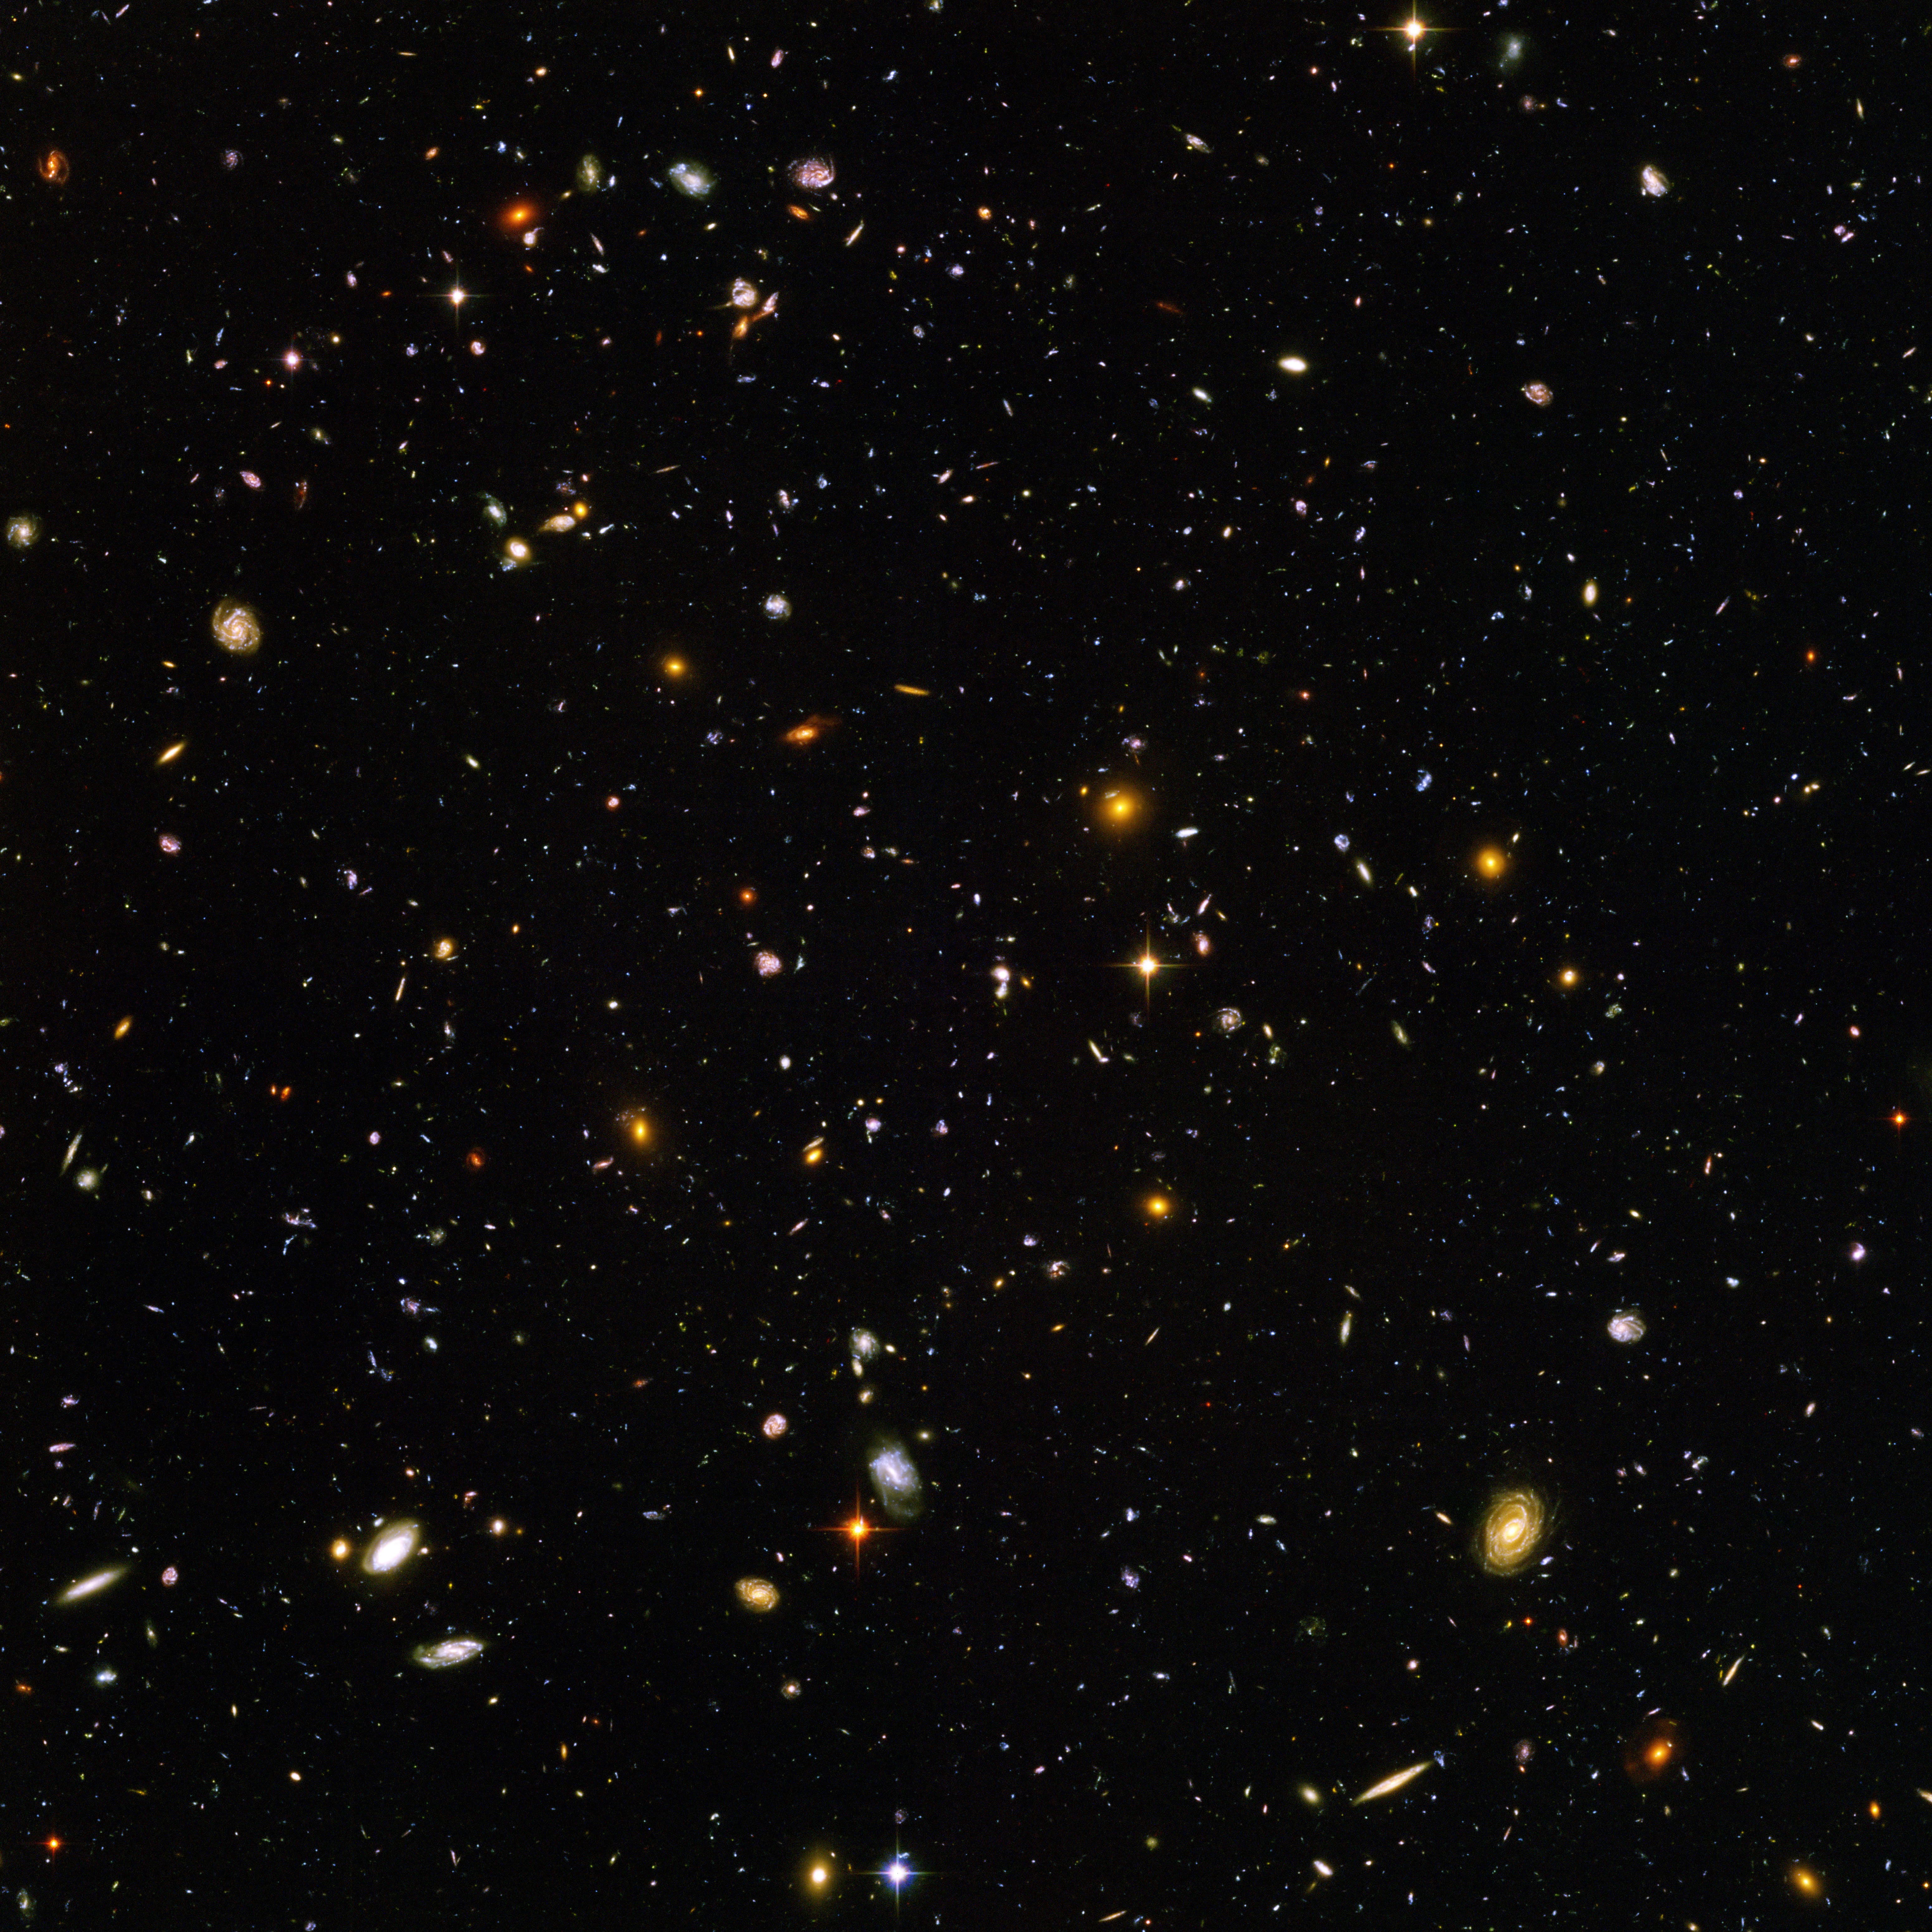
\includegraphics[width=13cm]{Images/Hubble_ultra_deep_field_high.jpg}
    \caption[Hubble ultra-deep field. (short name for list of figures)]{Hubble Ultra-Deep Field, in the constellation Fornax, 2004. Used with permission from NASA and the European Space Agency. Public Domain, https://commons.wikimedia.org/w/index.php?curid=5276968}
    \label{fig:hubble_deep_field}
\end{figure}

Detecting exoplanets itself has been a major recent scientific achievement, but with their existence confirmed, many studies have now moved their focus to attempting to characterize them. We can broadly assign categories (e.g. small rocky planets, hot Jupiters, water worlds) and carry out population-level studies to determine how frequently each type occurs.

\subsection{Etc}

More about your science.

\section{Thesis Structure}

The remainder of this thesis is structured as follows. Chapter~\ref{chapter:methods} introduces methods of science -- the methods introduced here are fundamental across several other Chapters. Chapter~\ref{chapter:science1} explores science. Chapter \ref{chapter:science2} presents even more science. In Chapter~\ref{chapter:science3} -- who would have guessed -- there is even more even more science. Finally, Chapter~\ref{chapter:conclusions} reflects on the thesis as a whole and concludes.